dal problema all'algoritmo 

\begin{itemize}
\item  propriet\`a dell'algoritmo
    \begin{itemize}
    \item non ambiguo
    \item deterministico
    \item termina in un numero finito di passi
   	\end{itemize}	
\item  tipologia di istruzioni
    \begin{itemize}
    \item istruzioni effettive
    \item istruzioni di controllo
    \end{itemize}   
\end{itemize}

diagrammi di flusso

\begin{itemize}
\item  blocchi elementari
    \begin{itemize}
    \item inizio
    \item fine
    \item istruzioni semplici
    \item visualizzazione risultati
    \item blocco di selezione
    \end{itemize}   
\end{itemize}

\mysep{}

\subsection{Tempo espresso in ore, minuti e secondi}
Si realizzi l'algoritmo che acquisito un valore intero (senz'altro positivo) che rappresenta una quantit\`a di tempo espressa in secondi, di calcola e visualizza la stessa quantit\`a di tempo espressa in ore, minuti e secondi. Per esempio, se si inserisce 3812, l'algoritmo calcola e visualizza 1 (ora) 3 (minuti) 32 (sec).

\begin{center}
    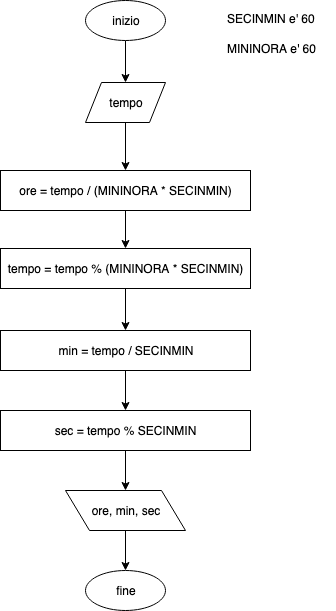
\includegraphics[width=0.3\textwidth]{./tempo.png}
\end{center}


\subsection{Operazioni di somma e sottrazione in modulo e segno}
Si realizzi l'algoritmo che acquisito un operatore (\texttt{'+'} o \texttt{'-'}) e due operandi effettua l'operazione e visualizza il risultato.

\begin{center}
    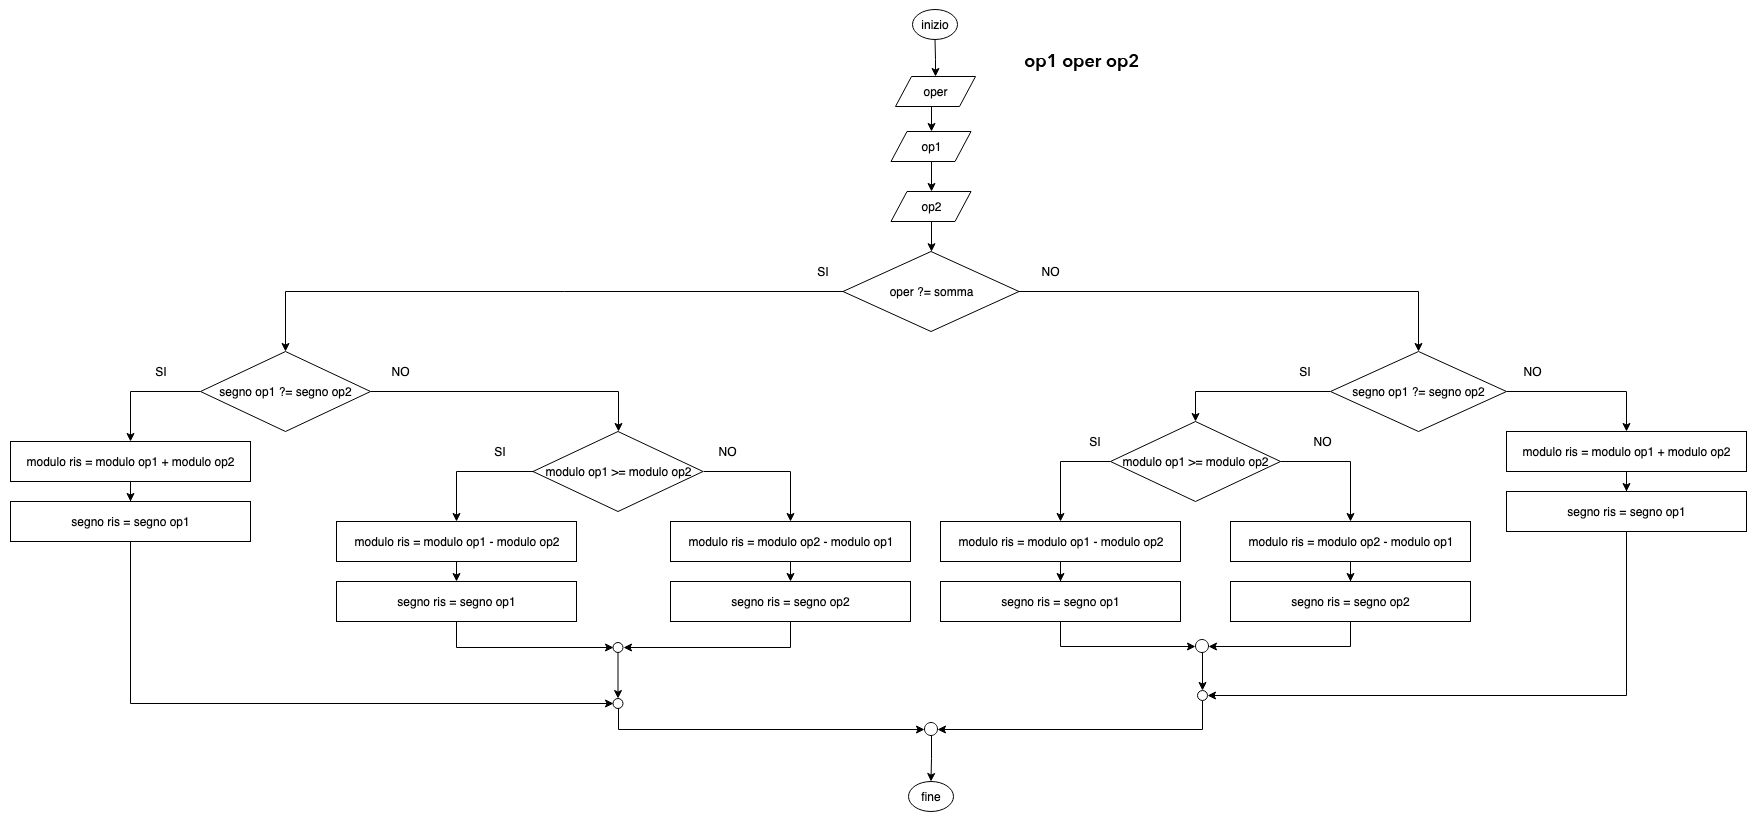
\includegraphics[width=0.9\textwidth]{./sommamodulosegno.png}
\end{center}


\subsection{Valore assoluto}
Si realizzi l'algoritmo che acquisito un valore intero calcola e visualizza il suo valore assoluto.

\begin{center}
    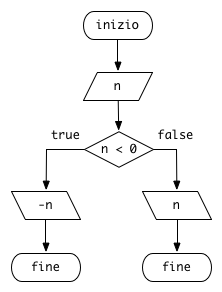
\includegraphics[width=0.3\textwidth]{./abs-alg1.png}
\end{center}

In questo caso l'algoritmo non calcola il valore assoluto, ma lo visualizza direttamente. Guardando la soluzione come una scatola nera, si ottiene il risultato richiesto, quindi soddisfa il comportamento atteso. Non rispetta la richiesta di calcolare il valore e poi visualizzarlo, ma questo aspetto \`e invisibile esternamente.
Ci sono pi\`u \texttt{fine}, aspetto poco pulito perch\'e diventa difficile riconciliare l'algoritmo.

\begin{center}
    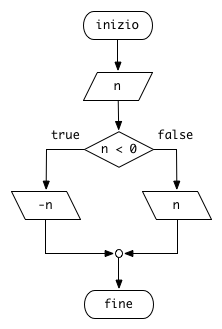
\includegraphics[width=0.3\textwidth]{./abs-alg2.png}
\end{center}

Anche in questo caso non si calcola il valore assoluto, ma si visualizza il risultato. \`E pi\`u pulito l'utilizzo di un unico punto di \texttt{fine}.

\begin{center}
    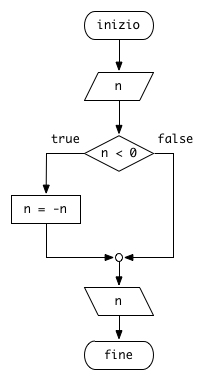
\includegraphics[width=0.3\textwidth]{./abs-alg3.png}
\end{center}

Questo algoritmo effettivamente calcola il valore assoluto e poi lo visualizza. Di fatto sovrascrive il valore iniziale con il valore assoluto, quindi eventualmente si perde questa informazione. Dal punto di vista della scatola nera, anche questa soluzione fa ci\`o che \`e richiesto.

\begin{center}
    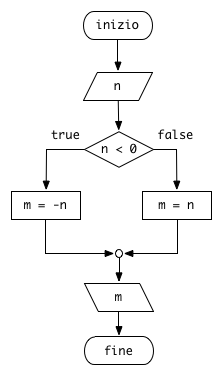
\includegraphics[width=0.3\textwidth]{./abs-alg4.png}
\end{center}

Questo algoritmo ha il comportamento richiesto e non perde il dato iniziale. L'approccio \`e migliore non tanto in relazione allo specifico problema (estremamente semplice) ma in termini di ``buone'' soluzioni, considerando che\begin{itemize} 
\item pu\`o essere necessario non tanto visualizzare il valore assoluto, ma utilizzarlo per ulteriori computazioni
\item il ``costo'' di un elemento in pi\`u per memorizzare il valore assoluto \`e irrisorio.
\end{itemize}
